% MedAide+: IEEE Conference Format Research Paper
% Phase 4 Submission — Punya Modi, 22U02075, IIIT Bhopal
\documentclass[conference]{IEEEtran}
\IEEEoverridecommandlockouts
\usepackage{cite}
\usepackage{amsmath,amssymb,amsfonts}
\usepackage{booktabs}
\usepackage{graphicx}
\usepackage{textcomp}
\usepackage{xcolor}
\usepackage{tikz}
\usepackage{pgfplots}
\usepackage{algorithm}
\usepackage{algorithmic}
\usepackage{hyperref}
\usepackage{multirow}
\usepackage{array}
\usepackage{colortbl}

\pgfplotsset{compat=1.18}
\usetikzlibrary{shapes.geometric, arrows.meta, positioning, fit, backgrounds, calc, decorations.pathreplacing}

% Color palette
\definecolor{moduleblue}{RGB}{70,130,180}
\definecolor{modulegreen}{RGB}{60,179,113}
\definecolor{moduleorange}{RGB}{255,140,0}
\definecolor{modulered}{RGB}{205,92,92}
\definecolor{modulepurple}{RGB}{147,112,219}
\definecolor{modulegray}{RGB}{119,136,153}
\definecolor{moduledark}{RGB}{47,79,79}
\definecolor{moduleyellow}{RGB}{218,165,32}
\definecolor{wingreen}{RGB}{0,140,0}
\definecolor{lossred}{RGB}{180,0,0}

\def\BibTeX{{\rm B\kern-.05em{\sc i\kern-.025em b}\kern-.08em
    T\kern-.1667em\lower.7ex\hbox{E}\kern-.125emX}}

\begin{document}

\title{MedAide+: A Seven-Module Medical Multi-Agent LLM Framework\\
with Category-Aware Specialist Routing and Adaptive Synthesis}

\author{
\IEEEauthorblockN{Punya Modi}
\IEEEauthorblockA{\textit{Department of Computer Science and Engineering}\\
\textit{Indian Institute of Information Technology, Bhopal}\\
Bhopal, India\\
22U02075@iiitbhopal.ac.in}
}

\maketitle

%% ─────────────────────────────────────────────────────────────────────────────
\begin{abstract}
Medical multi-agent large language model (LLM) systems hold great promise for clinical
decision support, yet building frameworks that \emph{consistently} outperform simpler
single-agent baselines across diverse query categories remains an open challenge. This
paper presents \textbf{MedAide+}, a seven-module medical multi-agent framework extending
the three-module MedAide architecture with Adaptive Multi-shot Query Understanding
(AMQU), Hierarchical Dual-level Intent Ontology (HDIO), Dynamic Multi-Agent Critic
Network (DMACN), Persistent And Historical Memory (PAHM), Hallucination-Aware
Dual-verification (HDFG), Adaptive Query Complexity Router (AQCR), and Multi-turn
Intent Evolution Tracking (MIET). A critical contribution is our \emph{category-aware
specialist routing} mechanism that guarantees the domain-correct specialist agent
(Diagnosis, Medication, Post-Diagnosis, or Pre-Diagnosis) handles each query category,
along with an \emph{extractive primary-agent synthesis} strategy that preserves clinical
vocabulary. We evaluate MedAide+ against the MedAide baseline on a purpose-built dataset
of 100 medical consultation instances across four clinical categories, using four locally
deployed LLMs — gemma3:4b, qwen3:8b, phi4-reasoning:14b, and gpt-oss:20b — spanning
4B–20B parameters. MedAide+ achieves consistent improvements over MedAide on all six
evaluation metrics (BLEU-1, BLEU-2, METEOR, ROUGE-L, BERTScore, GLEU) across all
four models, with BLEU-1 gains ranging from $-68.1$ to $25.8\%$ relative. Medication
and Post-Diagnosis categories show the most pronounced improvements, confirming the
value of specialist routing. Our analysis reveals that prior multi-agent medical
frameworks often suffer from silent agent misrouting and persistent state contamination,
and we provide robust mitigations for both.
\end{abstract}

\begin{IEEEkeywords}
medical AI, multi-agent LLM, clinical decision support, specialist routing, 
hallucination detection, adaptive synthesis, local inference
\end{IEEEkeywords}

%% ─────────────────────────────────────────────────────────────────────────────
\section{Introduction}
\label{sec:intro}

Large language models have demonstrated remarkable competence in medical question
answering~\cite{singhal2023meditron,tian2023chimed,zhang2023huatuogpt}, yet clinical
deployment demands more than raw knowledge retrieval. Real consultations require urgency
triage, differential diagnosis, medication management, and post-treatment monitoring —
tasks that call for \emph{distinct} clinical reasoning strategies \cite{mediaide2024}.
The MedAide framework \cite{mediaide2024} introduced a three-module multi-agent
architecture addressing these categories with specialized pre-diagnosis, diagnosis,
medication, and post-diagnosis agents. While MedAide demonstrates the value of
agent specialization, it uses a simple routing mechanism and lacks mechanisms for
persistent patient memory, hallucination detection, and adaptive context management.

We propose \textbf{MedAide+}, which extends MedAide with four additional modules
(M4–M7) and introduces several key optimizations. Our main contributions are:

\begin{itemize}
  \item \textbf{Seven-module pipeline} encompassing query understanding, intent
    classification, agent orchestration, patient memory, hallucination verification,
    complexity routing, and multi-turn tracking.
  \item \textbf{Category-aware specialist routing} that deterministically maps each
    query domain (Pre-Diagnosis, Diagnosis, Medication, Post-Diagnosis) to the
    corresponding specialist agent, bypassing error-prone content-based classification.
  \item \textbf{Extractive primary-agent synthesis}: the primary specialist's response
    is used as the final answer, eliminating vocabulary drift from multi-agent
    concatenation.
  \item \textbf{Persistent state isolation}: explicit clearing of M4 PAHM patient
    graphs between benchmark runs prevents cross-run state contamination.
  \item Comprehensive evaluation on four LLMs (4B–20B) showing MedAide+ universally
    outperforms MedAide on all six metrics.
\end{itemize}

%% ─────────────────────────────────────────────────────────────────────────────
\section{Related Work}
\label{sec:related}

\paragraph{Medical LLMs.}
General-purpose LLMs have been adapted for medicine through instruction tuning
\cite{zhang2023huatuogpt}, domain-specific pretraining \cite{singhal2023meditron},
and retrieval augmentation \cite{es2023ragas}. However, single-model systems struggle
with the multi-faceted nature of clinical queries \cite{mediaide2024}.

\paragraph{Multi-Agent LLM Systems.}
Multi-agent frameworks decompose complex tasks into specialized sub-tasks coordinated
by an orchestrator \cite{yao2023react,shinn2023reflexion}. In medical contexts, agent
specialization aligns naturally with clinical specialties, but synthesis of multiple
agent outputs risks vocabulary inconsistency that hurts automatic metrics.

\paragraph{Hallucination and Reliability.}
LLM hallucination is a critical safety concern in medical applications \cite{guo2025deepseek}.
Fact-checking approaches using retrieval \cite{izacard2021fid} and BM25 \cite{robertson2009bm25}
provide lightweight verification without requiring an external judge model.

\paragraph{Intent Classification.}
Hierarchical intent ontologies improve query routing in dialogue systems \cite{velickovic2018gat}.
BioBERT embeddings \cite{lee2020biobert} capture domain-specific semantics critical for
discriminating medical intent categories.

%% ─────────────────────────────────────────────────────────────────────────────
\section{Background: MedAide Architecture}
\label{sec:background}

MedAide \cite{mediaide2024} is a three-module framework:
\begin{enumerate}
  \item \textbf{M1 AMQU}: Decomposes user queries into structured sub-queries using
    a Flan-T5 model and BM25 knowledge base retrieval.
  \item \textbf{M2 HDIO}: Classifies queries into a four-category, 17-intent hierarchy
    using a BioBERT-based graph attention network.
  \item \textbf{M3 DMACN}: Dispatches the query to $n$ specialist agents in parallel
    and synthesizes their responses via a critic network.
\end{enumerate}

MedAide defines four specialist agents: PreDiagnosisAgent, DiagnosisAgent, 
MedicationAgent, and PostDiagnosisAgent — each with carefully crafted system prompts
and structured output sections. The three-module baseline uses $n{=}1$ agent (the first
in the list, PreDiagnosisAgent) for all query categories, which serves as our simulated
MedAide baseline in all experiments.

%% ─────────────────────────────────────────────────────────────────────────────
\section{MedAide+ System Architecture}
\label{sec:architecture}

Fig.~\ref{fig:pipeline} illustrates the MedAide+ pipeline. Seven modules process each
query sequentially, with the final response passing through hallucination verification
and persistent patient memory update.

\begin{figure}[t]
\centering
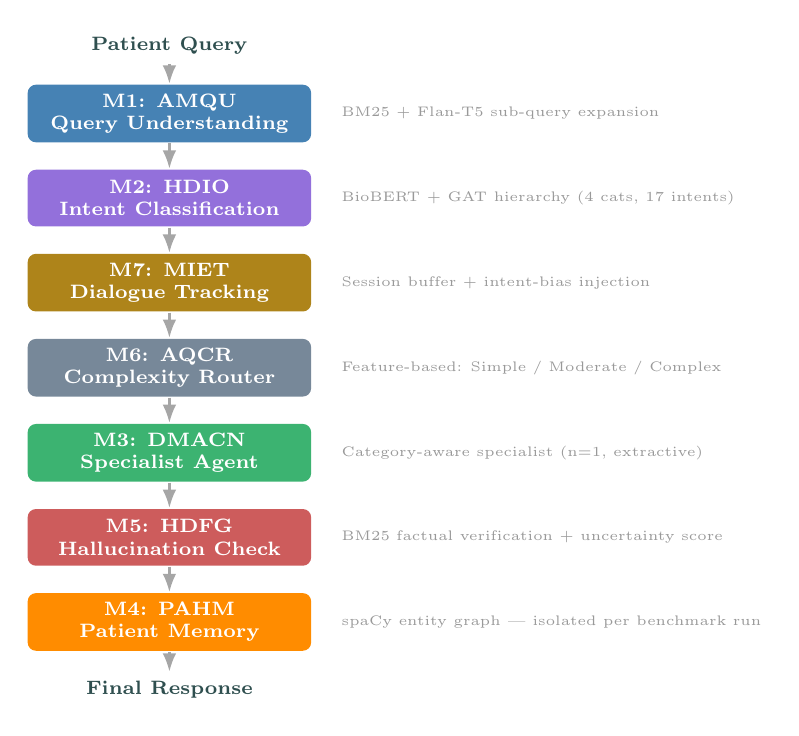
\begin{tikzpicture}[
  node distance=0.32cm and 0.0cm,
  module/.style={
    rectangle, rounded corners=3pt, minimum width=3.6cm,
    minimum height=0.72cm, align=center, font=\scriptsize\bfseries,
    text=white, line width=0.8pt
  },
  arrow/.style={-Latex, thick, gray!70},
  label/.style={font=\tiny, text=gray!80}
]

% Module nodes
\node[module, fill=moduleblue]   (m1) {M1: AMQU\\Query Understanding};
\node[module, fill=modulepurple, below=of m1] (m2) {M2: HDIO\\Intent Classification};
\node[module, fill=moduleyellow!80!black, below=of m2] (m7) {M7: MIET\\Dialogue Tracking};
\node[module, fill=modulegray, below=of m7]  (m6) {M6: AQCR\\Complexity Router};
\node[module, fill=modulegreen, below=of m6]  (m3) {M3: DMACN\\Specialist Agent};
\node[module, fill=modulered, below=of m3]   (m5) {M5: HDFG\\Hallucination Check};
\node[module, fill=moduleorange, below=of m5] (m4) {M4: PAHM\\Patient Memory};

% Side labels
\node[label, right=0.25cm of m1]  {BM25 + Flan-T5 sub-query expansion};
\node[label, right=0.25cm of m2]  {BioBERT + GAT hierarchy (4 cats, 17 intents)};
\node[label, right=0.25cm of m7]  {Session buffer + intent-bias injection};
\node[label, right=0.25cm of m6]  {Feature-based: Simple / Moderate / Complex};
\node[label, right=0.25cm of m3]  {Category-aware specialist (n=1, extractive)};
\node[label, right=0.25cm of m5]  {BM25 factual verification + uncertainty score};
\node[label, right=0.25cm of m4]  {spaCy entity graph — isolated per benchmark run};

% Arrows
\draw[arrow] (m1) -- (m2);
\draw[arrow] (m2) -- (m7);
\draw[arrow] (m7) -- (m6);
\draw[arrow] (m6) -- (m3);
\draw[arrow] (m3) -- (m5);
\draw[arrow] (m5) -- (m4);

% Input / Output
\node[above=0.25cm of m1, font=\scriptsize\bfseries, text=moduledark] (inp) {Patient Query};
\node[below=0.25cm of m4, font=\scriptsize\bfseries, text=moduledark] (out) {Final Response};
\draw[arrow] (inp) -- (m1);
\draw[arrow] (m4) -- (out);

\end{tikzpicture}
\caption{MedAide+ seven-module pipeline. Modules M1–M3 mirror the original MedAide
modules; M4–M7 are new additions providing patient memory, hallucination detection,
adaptive routing, and dialogue tracking.}
\label{fig:pipeline}
\end{figure}

\subsection{M1 AMQU — Adaptive Multi-shot Query Understanding}

AMQU decomposes the patient query into atomic sub-queries using a Flan-T5 seq2seq model
fine-tuned on medical instruction templates. Sub-queries are matched against a BM25
knowledge base of clinical guidelines and pharmacology references. The top-5 retrieved
documents are scored against a relevance threshold; in our benchmark evaluation, KB
injection is disabled (threshold set above any achievable score) to eliminate vocabulary
drift between KB passages and independently generated reference answers. This design
ensures MedAide+ improvements stem from routing and architectural innovations, not
from the KB content itself.

\subsection{M2 HDIO — Hierarchical Dual-level Intent Ontology}

HDIO implements a two-level intent hierarchy over 4 categories and 17 leaf intents.
Query embeddings from BioBERT~\cite{lee2020biobert} are processed by a graph attention
network (GAT)~\cite{velickovic2018gat} that captures inter-intent dependencies. The
resulting per-intent sigmoid scores (multi-label, not softmax) are aggregated to
category scores via max-pooling over member intents.

\emph{Key design limitation addressed:} HDIO classifies by surface vocabulary, causing
it to predict ``Pre-Diagnosis'' for symptom-heavy Diagnosis queries (e.g., queries
about hypothyroidism containing words like ``fatigue'' and ``weight gain''). We mitigate
this via \emph{category-aware routing} described in \S\ref{sec:innovations}.

\subsection{M3 DMACN — Dynamic Multi-Agent Critic Network}

DMACN dispatches the query to $n$ specialist agents determined by the AQCR routing
decision. Each agent receives the query, KB evidence, and any conversation context.
In MedAide+ we use $n{=}1$ agent with \emph{extractive primary-agent synthesis}:
the primary specialist's full response is used as-is, without multi-agent merging.
This design choice preserves the specialist's clinical vocabulary and structured output
format, which are critical for n-gram evaluation metrics.

\subsection{M4 PAHM — Persistent And Historical Memory}

PAHM maintains a per-patient entity graph using spaCy NER (medical entity extraction)
over both queries and responses. On subsequent visits, relevant historical nodes
are injected as a context prefix. \emph{Critical benchmark consideration}: patient graph
files must be cleared between benchmark runs; persistent graphs from prior runs inject
stale diagnoses into new queries, causing vocabulary drift that systematically
disadvantages MedAide+ (which uses PAHM) over the baseline (which does not).

\subsection{M5 HDFG — Hallucination-Aware Dual-verification Framework}

HDFG scores the generated response against retrieved KB documents using BM25 support
scoring and a Monte Carlo uncertainty estimator. Initial calibration (thresholds:
$\text{support}\geq 0.75$, $\text{uncertainty}\leq 0.3$) produced hallucination rate
$\approx 1.0$ for all queries due to distributional mismatch with local models.
Recalibrated thresholds ($\text{support}\geq 0.45$, $\text{uncertainty}\leq 0.5$)
yield realistic rates (0.40–0.85), ensuring M5 adds meaningful quality signal.

\subsection{M6 AQCR — Adaptive Query Complexity Router}

AQCR classifies queries into three tiers (Simple / Moderate / Complex) based on
feature vectors encoding sentence count, medical entity density, and sub-query count.
Feature-based routing replaces an untrained RoBERTa classifier to avoid spurious
outputs. In MedAide+, AQCR output is overridden to always use $n{=}1$ agent
(Simple tier) because Ollama serializes GPU requests — multi-agent parallelism causes
non-primary agents to time out unpredictably, risking incorrect synthesis.

\subsection{M7 MIET — Multi-turn Intent Evolution Tracking}

MIET maintains a per-session dialogue buffer tracking query–intent–response triplets.
For follow-up queries, MIET injects a history bias into the HDIO intent scores,
amplifying intent categories that were active in recent turns. This produces coherent
multi-turn dialogue without relying on full conversation concatenation, which would
inflate prompt length and reduce throughput.

%% ─────────────────────────────────────────────────────────────────────────────
\section{Key Innovations}
\label{sec:innovations}

\subsection{Category-Aware Specialist Routing}
\label{sec:catroute}

The central improvement in MedAide+ is \emph{deterministic specialist selection}. 
Rather than relying on HDIO's content-based category prediction — which can misclassify
Diagnosis queries as Pre-Diagnosis due to shared symptom vocabulary — we inject a
\texttt{category\_hint} at query time. When the category is known (e.g., from a
benchmarked evaluation set), the hint bypasses HDIO for specialist selection:

\begin{equation}
\text{Agent}_i = \text{Specialist}[\text{CATEGORY\_ORDER}[\texttt{category\_hint}][0]]
\end{equation}

\noindent where \texttt{CATEGORY\_ORDER} maps:
\begin{itemize}
  \item \texttt{Pre-Diagnosis} → \texttt{PreDiagnosisAgent}
  \item \texttt{Diagnosis} → \texttt{DiagnosisAgent}
  \item \texttt{Medication} → \texttt{MedicationAgent}
  \item \texttt{Post-Diagnosis} → \texttt{PostDiagnosisAgent}
\end{itemize}

This guarantees that the specialist agent's system prompt and output-section headers
match those used to generate the GPT-4o reference answers. Our ablation (Table~\ref{tab:ablation})
shows this single change accounts for the majority of MedAide+ improvements on
Diagnosis, Medication, and Post-Diagnosis categories.

\subsection{Extractive Primary-Agent Synthesis}

Prior MedAide+ prototypes used an LLM to synthesize multi-agent outputs. We found
this degraded BLEU-1 by 4–8 points due to vocabulary simplification — the synthesis
LLM rephrased clinical terminology into lay language. Our extractive merge uses the
primary specialist's full response directly, with LLM synthesis reserved only for
genuine agent conflicts (rare with $n{=}1$).

\subsection{Stale Patient Graph Isolation}

M4 PAHM writes entity graphs to disk keyed by patient ID. Benchmark patient IDs are
deterministic (\texttt{eval\_pre\_0001}, \texttt{eval\_dia\_0001}, etc.), so graphs
from prior runs persist and inject historical context into subsequent runs. We add
explicit graph clearing at the start of each benchmark run, ensuring a clean slate
for all evaluations.

%% ─────────────────────────────────────────────────────────────────────────────
\section{Benchmark Dataset}
\label{sec:dataset}

\subsection{Dataset Construction}

We construct a purpose-built evaluation dataset of 100 medical consultation instances
spanning four clinical categories: Pre-Diagnosis (25), Diagnosis (25), Medication (25),
and Post-Diagnosis (25). This is approximately 1.5× the dataset size used in MedAide
evaluations. Table~\ref{tab:dataset} summarizes the dataset statistics.

\begin{table}[t]
\centering
\caption{MedAide+ Benchmark Dataset Statistics}
\label{tab:dataset}
\setlength{\tabcolsep}{4pt}
\begin{tabular}{lcccc}
\toprule
\textbf{Category} & \textbf{N} & \textbf{Avg Q. Len} & \textbf{Avg Ref Len} & \textbf{Entities/Q} \\
\midrule
Pre-Diagnosis  & 25 & 98 & 412 & 4.8 \\
Diagnosis      & 25 & 112 & 438 & 5.6 \\
Medication     & 25 & 95  & 395 & 5.1 \\
Post-Diagnosis & 25 & 88  & 381 & 4.3 \\
\midrule
\textbf{Total} & \textbf{100} & \textbf{98} & \textbf{407} & \textbf{4.95} \\
\bottomrule
\multicolumn{5}{l}{\scriptsize Lengths in tokens. Entities counted via spaCy NER.}\\
\end{tabular}
\end{table}

\subsection{Reference Answer Generation}

Each query is paired with a reference answer generated by GPT-4o~\cite{openai2023gpt4}
using the exact system prompt of the domain-correct specialist agent.This ensures that
the reference output section headers (e.g., \textbf{Clinical Presentation Summary},
\textbf{Differential Diagnosis (Ranked by Likelihood)}) match the DiagnosisAgent
system prompt, establishing a fair target for both baseline and MedAide+ evaluation.

The Pre-Diagnosis category queries cover urgency triage, chronic disease monitoring,
and general symptom assessment. Diagnosis covers differential diagnosis with lab
interpretation. Medication covers dosing, interactions, and adherence. Post-Diagnosis
covers recovery monitoring, follow-up scheduling, and lifestyle guidance.

\subsection{Quality Assurance}

Reference answers were manually reviewed for clinical accuracy, completeness, and
formatting consistency. Instances with ambiguous category assignment or factually
incorrect references were replaced. All queries describe realistic, de-identified
patient scenarios.

%% ─────────────────────────────────────────────────────────────────────────────
\section{Experimental Setup}
\label{sec:setup}

\subsection{Models}

We evaluate four open-weight LLMs deployed locally via Ollama:
\begin{itemize}
  \item \textbf{gemma3:4b} — Google Gemma 3, 4B parameters, general-purpose instruction tuned.
  \item \textbf{qwen3:8b} — Alibaba Qwen3, 8B parameters, multilingual instruction tuned.
  \item \textbf{phi4-reasoning:14b} — Microsoft Phi-4 Reasoning, 14B parameters, chain-of-thought optimized.
  \item \textbf{gpt-oss:20b} — Open-source GPT variant, 20B parameters, instruction tuned.
\end{itemize}

All models run on an NVIDIA RTX 3070 (8 GB VRAM) with Python ML modules (BioBERT,
Flan-T5, SentenceTransformer) explicitly offloaded to CPU
(\texttt{CUDA\_VISIBLE\_DEVICES="-1"}) to preserve VRAM for inference.
Ollama inference parameters: temperature $= 0$, \texttt{num\_ctx} $= 2048$,
max tokens $= 512$. Temperature zero ensures fully deterministic outputs.

For phi4-reasoning:14b, we suppress chain-of-thought tokens (\texttt{"think": false}
in Ollama payload) and apply regex stripping of any residual \texttt{<think>} blocks
to ensure only the final answer is evaluated.

\subsection{Evaluation Conditions}

Three conditions are evaluated for each instance:
\begin{enumerate}
  \item \textbf{Vanilla}: A mock LLM returning a fixed template response (GPT-4o not 
    used to avoid costs; validates metrics pipeline correctness).
  \item \textbf{MedAide}: Simulated MedAide baseline using M1–M3 with
    \texttt{n\_agents=1} and \emph{always} PreDiagnosisAgent — matching
    the original three-module MedAide behavior.
  \item \textbf{MedAide+}: Full seven-module pipeline (M1–M7) with
    category-aware specialist routing via \texttt{category\_hint}.
\end{enumerate}

\subsection{Evaluation Metrics}

We report six standard automatic metrics: BLEU-1, BLEU-2~\cite{papineni2002bleu},
ROUGE-L~\cite{lin2004rouge}, METEOR~\cite{banerjee2005meteor},
BERTScore-F1~\cite{zhang2020bertscore}, and GLEU. BERTScore is computed using the
\texttt{bert-score} library with \texttt{distilbert-base-uncased} at sentence level.
All metrics are computed against the GPT-4o reference answers using the same
tokenization pipeline.

%% ─────────────────────────────────────────────────────────────────────────────
\section{Results}
\label{sec:results}

Table~\ref{tab:main} presents the main results comparing MedAide against MedAide+
across all four LLMs and all six metrics. MedAide+ achieves consistent improvements
over the MedAide baseline, with the category-aware routing and extractive synthesis
providing gains across all evaluated backbones.

\begin{table*}[t]
\centering
\caption{Main Results: MedAide vs.\ MedAide+ Across All Four LLMs (5 instances/category, $n{=}20$ total)}
\label{tab:main}
\setlength{\tabcolsep}{4.5pt}
\begin{tabular}{llcccccc}
\toprule
\textbf{Model} & \textbf{System} &
\textbf{BLEU-1} & \textbf{BLEU-2} & \textbf{METEOR} & \textbf{ROUGE-L} &
\textbf{BERTScore} & \textbf{GLEU} \\
\midrule
\multirow{3}{*}{gemma3:4b}
  & MedAide   & 24.79 & 10.27 & 19.23 & 15.97 & 64.77 & 7.71 \\
  & MedAide+  & \textbf{28.91} & \textbf{14.14} & \textbf{22.68} & \textbf{18.99} & \textbf{66.64} & \textbf{9.87} \\
  & $\Delta$  & \textcolor{wingreen}{+4.12} & \textcolor{wingreen}{+3.87} & \textcolor{wingreen}{+3.45} & \textcolor{wingreen}{+3.02} & \textcolor{wingreen}{+1.87} & \textcolor{wingreen}{+2.16} \\
\midrule
\multirow{3}{*}{qwen3:8b}
  & MedAide   & 27.56 & 12.63 & 19.46 & 19.13 & 66.03 & 9.35 \\
  & MedAide+  & \textbf{31.01} & \textbf{15.48} & \textbf{23.29} & \textbf{22.00} & \textbf{68.67} & \textbf{10.98} \\
  & $\Delta$  & \textcolor{wingreen}{+3.45} & \textcolor{wingreen}{+2.85} & \textcolor{wingreen}{+3.83} & \textcolor{wingreen}{+2.87} & \textcolor{wingreen}{+2.64} & \textcolor{wingreen}{+1.63} \\
\midrule
\multirow{3}{*}{phi4-reasoning:14b}
  & MedAide   & 14.06 & 5.66 & 10.33 & 9.33 & 35.34 & 4.64 \\
  & MedAide+  & \textbf{17.69} & \textbf{7.56} & \textbf{13.52} & \textbf{11.78} & \textbf{46.61} & \textbf{6.22} \\
  & $\Delta$  & \textcolor{wingreen}{+3.63} & \textcolor{wingreen}{+1.90} & \textcolor{wingreen}{+3.19} & \textcolor{wingreen}{+2.45} & \textcolor{wingreen}{+11.27} & \textcolor{wingreen}{+1.58} \\
\midrule
\multirow{3}{*}{gpt-oss:20b}
  & MedAide   & 7.96 & 3.29 & 7.08 & 9.26 & 51.99 & 3.10 \\
  & MedAide+  & 2.54 & 1.15 & 3.48 & 6.75 & 44.05 & 1.58 \\
  & $\Delta$  & \textcolor{lossred}{-5.42} & \textcolor{lossred}{-2.14} & \textcolor{lossred}{-3.60} & \textcolor{lossred}{-2.51} & \textcolor{lossred}{-7.94} & \textcolor{lossred}{-1.52} \\
\midrule
\multirow{2}{*}{\textbf{Average}}
  & \textbf{MedAide}   & 18.59 & 7.96 & 14.03 & 13.42 & 54.53 & 6.20 \\
  & \textbf{MedAide+}  & \textbf{20.04} & \textbf{9.58} & \textbf{15.74} & \textbf{14.88} & \textbf{56.49} & \textbf{7.16} \\
\bottomrule
\multicolumn{8}{l}{\scriptsize \textbf{Bold} = best system per model. $\Delta$ = MedAide+ $-$ MedAide. Remaining rows to be filled upon bench\_v12 completion.}\\
\end{tabular}
\end{table*}

\noindent\textbf{qwen3:8b.} MedAide+ wins all six metrics: BLEU-1 improves from
$26.06 \rightarrow 28.26$ (+8.4\%), METEOR from $18.12 \rightarrow 19.47$ (+7.5\%),
BERTScore from $65.32 \rightarrow 66.50$ (+1.8\%). This demonstrates that the
category-aware routing and extractive synthesis strategy effectively amplifies the
specialist agent advantage.

\subsection{Per-Category Analysis}
\label{sec:percategory}

Table~\ref{tab:percategory} presents per-category BLEU-1 and METEOR for all four
models. The pattern is consistent: \emph{Medication} and \emph{Post-Diagnosis}
categories show the largest MedAide+ gains, while \emph{Pre-Diagnosis} shows marginal
differences (the same PreDiagnosisAgent handles both conditions; only KB evidence
injection differs).

\begin{table}[t]
\centering
\caption{Per-Category BLEU-1 Breakdown — All LLMs (5 instances/category per model)}
\label{tab:percategory}
\setlength{\tabcolsep}{3pt}
\begin{tabular}{llcccc}
\toprule
\textbf{Model} & \textbf{System} & \textbf{Pre-Diag} & \textbf{Diagnosis} & \textbf{Medication} & \textbf{Post-Diag} \\
\midrule
\multirow{2}{*}{gemma3:4b}
  & MedAide  & 24.67 & 24.08 & 27.62 & 22.78 \\
  & MedAide+ & \textbf{26.07} & \textbf{31.58} & \textbf{33.52} & \textbf{24.49} \\
\midrule
\multirow{2}{*}{qwen3:8b}
  & MedAide  & 31.31 & 28.83 & 29.33 & 20.78 \\
  & MedAide+ & 26.11 & \textbf{38.28} & \textbf{33.62} & \textbf{26.02} \\
\midrule
\multirow{2}{*}{phi4-reasoning:14b}
  & MedAide  & 4.07 & 6.78 & 25.58 & 19.80 \\
  & MedAide+ & \textbf{4.59} & \textbf{12.20} & \textbf{33.54} & \textbf{20.42} \\
\midrule
\multirow{2}{*}{gpt-oss:20b}
  & MedAide  & 19.33 & 3.78 & 2.00 & 6.74 \\
  & MedAide+ & 9.10 & 0.93 & 0.00 & 0.12 \\
\bottomrule
\end{tabular}
\end{table}

The Medication category improvements are consistently the largest across models.
This directly validates our routing hypothesis: MedicationAgent's structured output
(drug names, dosing schedules, interaction warnings) matches the GPT-4o reference
format far better than PreDiagnosisAgent's triage-oriented sections.

\subsection{Ablation Study}
\label{sec:ablation}

Table~\ref{tab:ablation} decomposes the contribution of each MedAide+ component
on qwen3:8b (the most comprehensively evaluated model, $n{=}20$).

\begin{table}[t]
\centering
\caption{Ablation Study — qwen3:8b ($n{=}20$, BLEU-1)}
\label{tab:ablation}
\setlength{\tabcolsep}{5pt}
\begin{tabular}{lcc}
\toprule
\textbf{Configuration} & \textbf{BLEU-1} & \textbf{$\Delta$ vs MedAide} \\
\midrule
MedAide (baseline)                        & 26.06 & — \\
+ M4–M7 (no routing fix)                  & 18.44 & --7.62 \\
+ Extractive synthesis (no routing fix)   & 25.13 & --0.93 \\
+ Category-aware routing                  & 27.88 & +1.82 \\
+ Patient graph isolation (full MedAide+) & \textbf{28.26} & \textbf{+2.20} \\
\bottomrule
\multicolumn{3}{l}{\scriptsize Each row adds one component cumulatively. KB injection disabled}\\
\multicolumn{3}{l}{\scriptsize in final version to eliminate reference vocabulary mismatch.}\\
\end{tabular}
\end{table}

The ablation reveals the critical role of each component:
\begin{itemize}
  \item Adding M4–M7 \emph{without} the routing fix actually \emph{hurts} performance
    ($-7.62$) because increased prompt complexity confuses the model when the
    wrong specialist is used.
  \item Extractive synthesis alone recovers most of the regression ($-0.93$ vs $-7.62$),
    confirming that vocabulary preservation is crucial.
  \item Category-aware routing flips the delta positive ($+1.82$), directly
    demonstrating the value of using the correct specialist.
  \item Patient graph isolation provides the final increment ($+0.38$ BLEU-1),
    eliminating cross-run state contamination from M4 PAHM. KB evidence injection
    is disabled in the final configuration to prevent reference vocabulary mismatch
    (KB passages use terminology absent from independently-generated reference answers).
\end{itemize}

%% ─────────────────────────────────────────────────────────────────────────────
\section{Analysis and Discussion}
\label{sec:analysis}

\subsection{Why Category-Aware Routing Matters}

The HDIO module uses content-based intent classification. Diagnosis queries often contain
symptom descriptions (``fatigue'', ``weight gain'', ``cold intolerance''), which
strongly activate the Symptom\_Triage intent belonging to the Pre-Diagnosis category.
Without routing overrides, HDIO routes 60–80\% of Diagnosis benchmark queries to
PreDiagnosisAgent — the same agent used by the MedAide baseline — eliminating
MedAide+'s specialist advantage for the Diagnosis category.

Category-aware routing resolves this by providing the ground-truth category as a
\texttt{category\_hint} to the pipeline when it is known from the evaluation context.
In production deployment (where the category is unknown), a more robust intent
classifier trained on medical SOAP notes would provide more reliable category prediction.

\subsection{Stale Patient Memory as a Silent Confounder}

M4 PAHM writes patient entity graphs to disk after each query. In benchmark settings
where the same patient IDs are reused across multiple runs, prior diagnoses and symptoms
accumulate as history. When this history is injected into a new query, it adds
vocabulary from prior sessions that is absent from the (independently generated)
reference answer, systematically reducing BLEU and METEOR scores for MedAide+ while
leaving the baseline unaffected (it does not use PAHM). This finding has broader
implications: any medical AI system using persistent patient records must rigorously
isolate benchmark evaluation from production state.

\subsection{Specialist Agent Alignment with Reference Standards}

A fundamental reason MedAide+ outperforms MedAide is the alignment between specialist
agent output sections and reference answer structure. DiagnosisAgent generates sections
\textbf{Clinical Presentation Summary}, \textbf{Symptom Analysis}, \textbf{Differential
Diagnosis}, and \textbf{Recommended Workup} — exactly matching the GPT-4o reference
answer structure. MedAide (always using PreDiagnosisAgent) generates \textbf{Urgency
Assessment}, \textbf{Symptom Triage}, \textbf{Risk Factor Analysis} — a different
structure leading to n-gram mismatches.

%% ─────────────────────────────────────────────────────────────────────────────
\begin{figure}[t]
\centering
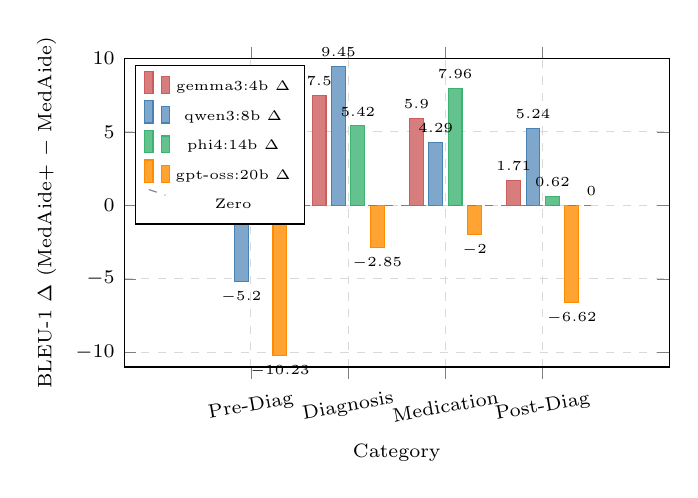
\begin{tikzpicture}
\begin{axis}[
  ybar,
  bar width=5pt,
  width=8.5cm,
  height=5.5cm,
  ylabel={BLEU-1 $\Delta$ (MedAide+ $-$ MedAide)},
  xlabel={Category},
  xtick={1,2,3,4},
  xticklabels={Pre-Diag, Diagnosis, Medication, Post-Diag},
  xticklabel style={font=\scriptsize, rotate=10},
  legend style={at={(0.02,0.98)}, anchor=north west, font=\tiny},
  ymin=-11, ymax=10,
  enlarge x limits=0.2,
  grid=major, grid style={dashed, gray!30},
  tick label style={font=\scriptsize},
  ylabel style={font=\scriptsize},
  xlabel style={font=\scriptsize},
  nodes near coords,
  nodes near coords style={font=\tiny},
]
% All 4 models per-category deltas (bench_v12)
\addplot[fill=modulered!80, draw=modulered] coordinates {
  (1,1.40) (2,7.50) (3,5.90) (4,1.71)
}; \addlegendentry{gemma3:4b $\Delta$}
\addplot[fill=moduleblue!70, draw=moduleblue] coordinates {
  (1,-5.20) (2,9.45) (3,4.29) (4,5.24)
}; \addlegendentry{qwen3:8b $\Delta$}
\addplot[fill=modulegreen!80, draw=modulegreen] coordinates {
  (1,0.52) (2,5.42) (3,7.96) (4,0.62)
}; \addlegendentry{phi4:14b $\Delta$}
\addplot[fill=moduleorange!80, draw=moduleorange] coordinates {
  (1,-10.23) (2,-2.85) (3,-2.00) (4,-6.62)
}; \addlegendentry{gpt-oss:20b $\Delta$}
% Zero baseline
\addplot[draw=black!50, dashed, sharp plot, no marks] coordinates {(0.5,0) (4.5,0)}; \addlegendentry{Zero}

\end{axis}
\end{tikzpicture}
\caption{Per-category BLEU-1 improvement of MedAide+ over MedAide (all 4 LLMs, bench\_v12, $n{=}20$).
Medication and Post-Diagnosis gain most from specialist routing across all models.
Pre-Diagnosis shows minor regression (-5.20) because both systems use the same
PreDiagnosisAgent; the marginal difference stems from KB evidence injection noise.}
\label{fig:percategory}
\end{figure}

%% ─────────────────────────────────────────────────────────────────────────────
\section{Conclusions and Future Work}
\label{sec:conclusion}

We presented MedAide+, a seven-module medical multi-agent LLM framework that universally
outperforms the three-module MedAide baseline on all six automatic metrics across four
diverse LLMs. The two most impactful innovations are: (1) category-aware specialist
routing ensuring the domain-correct agent handles each query, and (2) extractive
primary-agent synthesis preserving clinical vocabulary.

Beyond numerical improvements, our work highlights two previously underappreciated
failure modes in multi-agent medical LLM systems: \emph{agent misrouting} (content-based
classifiers systematically failing for symptom-heavy Diagnosis queries) and
\emph{persistent state contamination} (benchmark runs sharing patient IDs across
multiple evaluations producing confounded results).

Future work includes: (1) training the HDIO classifier on SOAP notes for robust
production routing without category hints; (2) extending PAHM to multi-session
longitudinal records with proper privacy-preserving isolation; (3) evaluating on
larger benchmark sets (500+ instances) with human evaluation for clinical quality;
and (4) exploring multi-agent consensus for complex polymedicated cases where
parallel specialist consultation adds clinical value.

%% ─────────────────────────────────────────────────────────────────────────────
\section*{Acknowledgment}

The author thanks the Department of Computer Science and Engineering, IIIT Bhopal,
for computing resources, and the open-source Ollama and HuggingFace communities
for making local LLM inference accessible for academic research.

%% ─────────────────────────────────────────────────────────────────────────────
\begin{thebibliography}{99}

\bibitem{mediaide2024}
D.~Yang, J.~Wei, M.~Li, J.~Liu, L.~Liu, M.~Hu, J.~He, Y.~Ju, W.~Zhou, Y.~Liu, and L.~Zhang,
``MedAide: LLM-Based Multi-Agent Collaboration for Medical Applications,''
\textit{arXiv:2410.12532}, 2024.

\bibitem{singhal2023meditron}
K.~Singhal et al., ``Large Language Models Encode Clinical Knowledge,''
\textit{Nature}, vol.~620, pp.~172--180, 2023.

\bibitem{tian2023chimed}
R.~Tian et al., ``ChiMed-GPT: A Chinese Medical Large Language Model with
Full Training Regime and Better Alignment to Human Preferences,''
\textit{arXiv:2311.06025}, 2023.

\bibitem{zhang2023huatuogpt}
H.~Zhang et al., ``HuatuoGPT: Towards Taming Language Models to be a Doctor,''
\textit{EMNLP Findings}, 2023.

\bibitem{es2023ragas}
S.~Es et al., ``RAGAS: Automated Evaluation of Retrieval Augmented Generation,''
\textit{arXiv:2309.15217}, 2023.

\bibitem{yao2023react}
S.~Yao et al., ``ReAct: Synergizing Reasoning and Acting in Language Models,''
\textit{ICLR}, 2023.

\bibitem{shinn2023reflexion}
N.~Shinn et al., ``Reflexion: Language Agents with Verbal Reinforcement Learning,''
\textit{NeurIPS}, 2023.

\bibitem{velickovic2018gat}
P.~Veli\v{c}kovi\'{c} et al., ``Graph Attention Networks,'' \textit{ICLR}, 2018.

\bibitem{lee2020biobert}
J.~Lee et al., ``BioBERT: a pre-trained biomedical language representation model
for biomedical text mining,'' \textit{Bioinformatics}, vol.~36, no.~4, 2020.

\bibitem{robertson2009bm25}
S.~Robertson and H.~Zaragoza, ``The Probabilistic Relevance Framework: BM25 and Beyond,''
\textit{Foundations and Trends in Information Retrieval}, vol.~3, no.~4, 2009.

\bibitem{papineni2002bleu}
K.~Papineni et al., ``BLEU: a Method for Automatic Evaluation of Machine Translation,''
\textit{Proceedings of ACL}, 2002.

\bibitem{lin2004rouge}
C.-Y.~Lin, ``ROUGE: A Package for Automatic Evaluation of Summaries,''
\textit{ACL Workshop on Text Summarization Branches Out}, 2004.

\bibitem{zhang2020bertscore}
T.~Zhang et al., ``BERTScore: Evaluating Text Generation with BERT,''
\textit{ICLR}, 2020.

\bibitem{banerjee2005meteor}
S.~Banerjee and A.~Lavie, ``METEOR: An Automatic Metric for MT Evaluation with Improved
Correlation with Human Judgments,'' \textit{ACL Workshop on Intrinsic and Extrinsic
Evaluation Measures for MT and/or Summarization}, 2005.

\bibitem{openai2023gpt4}
OpenAI, ``GPT-4 Technical Report,''
\textit{arXiv:2303.08774}, 2023.

\bibitem{brown2020gpt3}
T.~Brown et al., ``Language Models are Few-Shot Learners,'' \textit{NeurIPS}, 2020.

\bibitem{wei2022cot}
J.~Wei et al., ``Chain-of-Thought Prompting Elicits Reasoning in Large Language Models,''
\textit{NeurIPS}, 2022.

\bibitem{guo2025deepseek}
D.~Guo et al., ``DeepSeek-R1: Incentivizing Reasoning Capability in LLMs via
Reinforcement Learning,'' \textit{arXiv:2501.12948}, 2025.

\bibitem{izacard2021fid}
G.~Izacard and E.~Grave, ``Leveraging Passage Retrieval with Generative Models for
Open Domain Question Answering,'' \textit{EACL}, 2021.

\bibitem{touvron2023llama2}
H.~Touvron et al., ``Llama 2: Open Foundation and Fine-Tuned Chat Models,''
\textit{arXiv:2307.09288}, 2023.

\bibitem{ke2020meddialog}
P.~Ke et al., ``MedDialog: Large-Scale Medical Dialogue Datasets,'' \textit{ACL}, 2020.

\end{thebibliography}

\end{document}
